\chapter{Diseño e implementación} % Main chapter title

\label{Chapter3} % Change X to a consecutive number; for referencing this chapter elsewhere, use \ref{ChapterX}

\definecolor{mygreen}{rgb}{0,0.6,0}
\definecolor{mygray}{rgb}{0.5,0.5,0.5}
\definecolor{mymauve}{rgb}{0.58,0,0.82}

%%%%%%%%%%%%%%%%%%%%%%%%%%%%%%%%%%%%%%%%%%%%%%%%%%%%%%%%%%%%%%%%%%%%%%%%%%%%%
% parámetros para configurar el formato del código en los entornos lstlisting
%%%%%%%%%%%%%%%%%%%%%%%%%%%%%%%%%%%%%%%%%%%%%%%%%%%%%%%%%%%%%%%%%%%%%%%%%%%%%
\lstset{ %
  backgroundcolor=\color{white},   % choose the background color; you must add \usepackage{color} or \usepackage{xcolor}
  basicstyle=\footnotesize,        % the size of the fonts that are used for the code
  breakatwhitespace=false,         % sets if automatic breaks should only happen at whitespace
  breaklines=true,                 % sets automatic line breaking
  captionpos=b,                    % sets the caption-position to bottom
  commentstyle=\color{mygreen},    % comment style
  deletekeywords={...},            % if you want to delete keywords from the given language
  %escapeinside={\%*}{*)},          % if you want to add LaTeX within your code
  %extendedchars=true,              % lets you use non-ASCII characters; for 8-bits encodings only, does not work with UTF-8
  %frame=single,	                % adds a frame around the code
  keepspaces=true,                 % keeps spaces in text, useful for keeping indentation of code (possibly needs columns=flexible)
  keywordstyle=\color{blue},       % keyword style
  language=[ANSI]C,                % the language of the code
  %otherkeywords={*,...},           % if you want to add more keywords to the set
  numbers=left,                    % where to put the line-numbers; possible values are (none, left, right)
  numbersep=5pt,                   % how far the line-numbers are from the code
  numberstyle=\tiny\color{mygray}, % the style that is used for the line-numbers
  rulecolor=\color{black},         % if not set, the frame-color may be changed on line-breaks within not-black text (e.g. comments (green here))
  showspaces=false,                % show spaces everywhere adding particular underscores; it overrides 'showstringspaces'
  showstringspaces=false,          % underline spaces within strings only
  showtabs=false,                  % show tabs within strings adding particular underscores
  stepnumber=1,                    % the step between two line-numbers. If it's 1, each line will be numbered
  stringstyle=\color{mymauve},     % string literal style
  tabsize=2,	                   % sets default tabsize to 2 spaces
  title=\lstname,                  % show the filename of files included with \lstinputlisting; also try caption instead of title
  morecomment=[s]{/*}{*/}
}


%----------------------------------------------------------------------------------------
%	SECTION 1
%----------------------------------------------------------------------------------------
\section{Arquitectura del sistema embebido}
 
\section{Selección de componentes}

\section{Desarrollo de software}

INDICAR QUE EL SOFTWARE SE DESARROLLO PRIMERO EN PLACA DE DESARROLLO Y DESPUES SE IMPLEMENTO

\subsection{Driver CAN}

\subsection{Interfaz HMI}

\subsection{Interfaz UART-USB}

\section{Modificaciones firmware SN-17}

\section{Desarrollo de Hardware}

Para el desarrollo del hardware se utilizó el software de diseño Altium\footnote{\url{https://www.altium.com/}} y se eligió como fabricante a PCBWING\footnote{\url{https://www.pcbwing.com/}} que es una empresa con la que trabaja comúnmente Cambre ICyFSA. Se tomó, como punto de partida, las capacidades técnicas de este fabricante.

Se decidió hacer una placa de 4 capas, con dimensiones menores a 100 x 100 mm. Esto se debe a que el fabricante PCBWING ofrece precios más económicos para estas condiciones de fabricación y se consideró que no imponen restricciones importantes el diseño requerido.


\section{Desarrollo de gabinete}

Para el desarrollo del gabinete se usó el software de diseño Autodesk Inventor\footnote{\url{https://www.autodesk.com/products/inventor/overview?term=1-YEAR&tab=subscription}}. Se determinó armar un ensamble en que incluya todos los componentes y se lo pensó para poder luego ser impreso en 3D.

Para los componentes comprados, como la pantalla LCD y la matriz de botones, se tomaron los modelos 3D libres conseguidos a través de la plataforma GrabCAD\footnote{\url{https://grabcad.com/}}. Estos se verificaron para asegurarse que sus medidas correspondieran con el dispositivo físico. Por ultimo, el modelo de la plaqueta desarrollada se exportó desde el software Altium, donde se diseñó.

También, se priorizó el acceso a los conectores de la plaqueta, para permitir realizar cambios de cableados con poco esfuerzo, pero manteniendo los circuitos protegidos. Esto se puede ver en la Figura \ref{fig:ensamble} donde se muestra el ensamble completo en Inventor. Notar que las piezas superiores, donde están la pantalla y el teclado, se muestran transparentes, para ayudar con la visualización.

\begin{figure}[htbp]
	\centering
	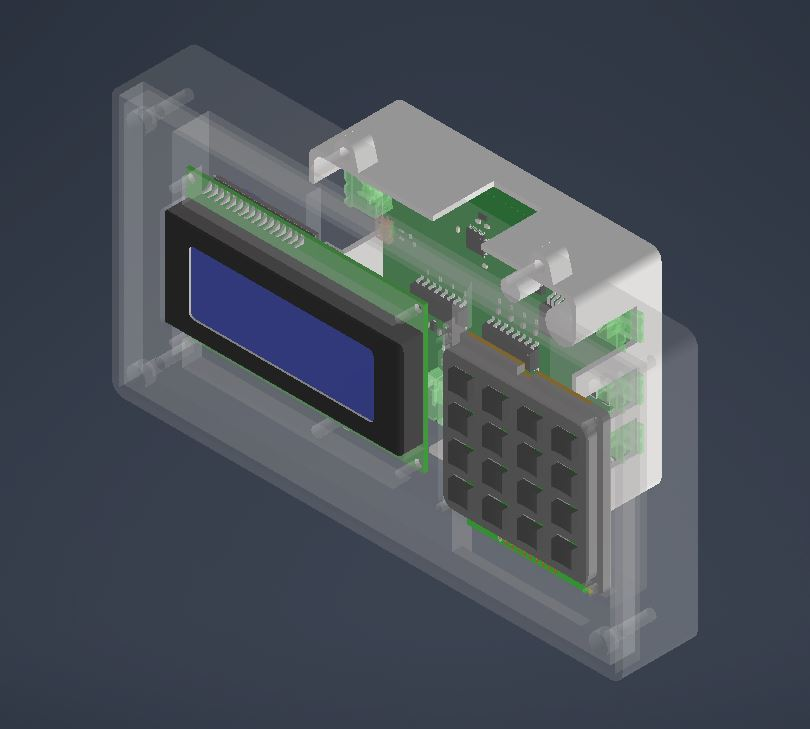
\includegraphics[scale=.6]{./Figures/asm_3d.JPG}
	\caption{Ensamble 3D de gabinete}
	\label{fig:ensamble}
\end{figure}

Como se puede ver, el ensamble consta de 3 componentes: una tapa delantera donde apoyan el display y el teclado, una caja intermedia que encierra a estos y una caja trasera donde se coloca la plaqueta de control. Se decidió por esta forma para permitir una presentación cómoda de los elementos de interfaz, para que el cableado interno quede protegido y para que se tenga fácil acceso a los conectores de la plaqueta, como se mecionó previamente.

Una vez cerrado el diseño, se exportó el archivo al programa UltiMaker Cura\footnote{\url{https://ultimaker.com/software/ultimaker-cura}}, donde se generaron los archivos de fabricación para impresión 3D. Se decidió utilizar PLA, que es uno de los plásticos más económicos y simples de manipular, y que cuenta con las características mecánicas apropiadas para la aplicación. Luego de fabricado, se forman las roscas en las distintas piezas y se ensambla el conjunto.